% Standalone figure for "Freysoldt's Review.tex" (Section 2).
% The lattice model: a crystal region with N sites in contact with a heat
% bath, atom reservoirs and an electron reservoir.
\documentclass[11pt,tikz,border=2pt]{standalone}
\usepackage{amsmath,amssymb}
\usetikzlibrary{arrows.meta, positioning}
\begin{document}
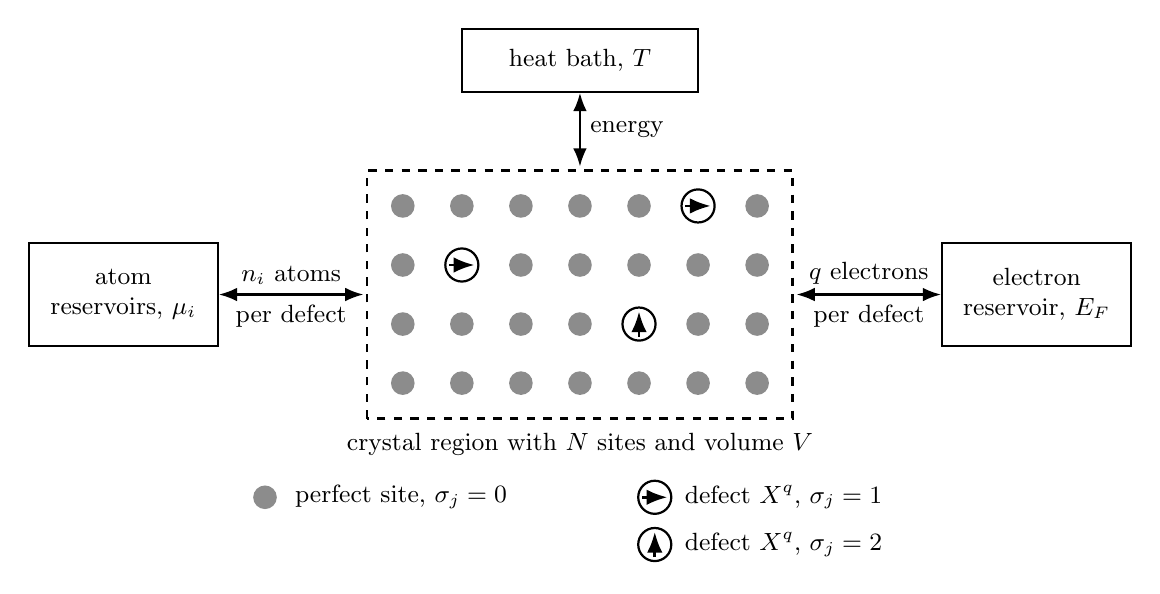
\begin{tikzpicture}[font=\small, >=Latex, line width=0.8pt]
  % ---- crystal region ----
  \def\a{0.75}
  \draw[dashed] (-0.45,-0.45) rectangle (4.95,2.70);
  \foreach \x in {0,...,6} {
    \foreach \y in {0,...,3} {
      \fill[black!45] (\x*\a,\y*\a) circle (0.15);
    }
  }
  % defect sites: open circle with an arrow for the internal state
  \foreach \x/\y/\ang in {1/2/0, 4/1/90, 5/3/0} {
    \fill[white] (\x*\a,\y*\a) circle (0.24);
    \draw (\x*\a,\y*\a) circle (0.21);
    \draw[->, line width=1.0pt] (\x*\a,\y*\a) ++(\ang:-0.16) -- ++(\ang:0.32);
  }
  \node[below] at (2.25,-0.50) {crystal region with $N$ sites and volume $V$};
  % ---- legend ----
  \fill[black!45] (-1.75,-1.45) circle (0.15);
  \node[right] at (-1.50,-1.45) {perfect site, $\sigma_j=0$};
  \draw (3.20,-1.45) circle (0.21);
  \draw[->, line width=1.0pt] (3.04,-1.45) -- (3.36,-1.45);
  \node[right] at (3.45,-1.45) {defect $X^q$, $\sigma_j=1$};
  \draw (3.20,-2.05) circle (0.21);
  \draw[->, line width=1.0pt] (3.20,-2.21) -- (3.20,-1.89);
  \node[right] at (3.45,-2.05) {defect $X^q$, $\sigma_j=2$};
  % ---- heat bath ----
  \node[draw, minimum width=3.0cm, minimum height=0.8cm] (bath) at (2.25,4.10) {heat bath, $T$};
  \draw[<->] (2.25,2.75) -- (bath.south) node[midway, right] {energy};
  % ---- atom reservoirs ----
  \node[draw, align=center, minimum width=2.4cm, minimum height=1.3cm] (atoms) at (-3.55,1.125)
       {atom\\reservoirs, $\mu_i$};
  \draw[<->] (atoms.east) -- (-0.50,1.125)
       node[midway, above] {$n_i$ atoms} node[midway, below] {per defect};
  % ---- electron reservoir ----
  \node[draw, align=center, minimum width=2.4cm, minimum height=1.3cm] (els) at (8.05,1.125)
       {electron\\reservoir, $E_F$};
  \draw[<->] (5.00,1.125) -- (els.west)
       node[midway, above] {$q$ electrons} node[midway, below] {per defect};
\end{tikzpicture}
\end{document}
